\begin{fact}\label{iso-tri}
	Considérons tous les triangles de périmètre fixé $p$. Parmi tous ces triangles, celui d'aire maximale est le triangle équilatéral de côté $c = \dfrac13 p$.
\end{fact}


\begin{proof}
	Une première idée, calculatoire, est de passer via la classique formule de Héron $Aire = \sqrt{s(s - a)(s - b)(s - c)}$ où $s = \num{.5} p$ désigne le demi-périmètre, et les variables $a$, $b$ et $c$ les mesures des côtés du triangle. 
	Comme l'aire est positive ou nulle, il suffit de chercher les maxima de $Aire^2 = s(s - a)(s - b)(s - c)$. La méthode des extrema liés s'appliquent ici,%
	\footnote{
		Nous devons trouver un éventuel maximum de $f(a;b;c) = \frac{1}{16} (a + b + c)(b + c - a)(a + c - b)(a + b - c)$ sous la contrainte $2s = a + b + c$ où $s > 0$ est une constante.
		Notant $g(a;b;c) = a + b + c - 2 s$, la contrainte s'écrit $g(a;b;c) = 0$.
		Selon la méthode des extrema liés, un éventuel maximum doit vérifier 
		$\pder[i]{f}{a}{1} = \lambda \pder[i]{g}{a}{1}$,
		$\pder[i]{f}{b}{1} = \lambda \pder[i]{g}{b}{1}$ et
		$\pder[i]{f}{c}{1} = \lambda \pder[i]{g}{c}{1}$
		pour un certain réel $\lambda$.
		Donc,
		$- s(s - b)(s - c) = - s(s - a)(s - c) = - s(s - a)(s - b) = \lambda$,
		puis
		$(s - b)(s - c) = (s - a)(s - c) = (s - a)(s - b)$.
		Le cas $s = a$, $s = b$ ou $s = c$ donne $f(a;b;c) = 0$ à chaque fois.
		Quant au cas $s \neq a$, $s \neq b$ et $s \neq c$, il n'est envisageable que si $a = b = c = \frac{p}{3}$ qui implique $f(a;b;c) = \frac{1}{16} p \big( \frac{p}{3} \big)^3 > 0$.
		En résumé, l'existence d'un maximum implique que ce maximum corresponde au cas du triangle équilatéral.
		Il reste à justifier qu'un tel maximum existe pour pouvoir conclure.
		Ceci est facile à justifier en considérant le compact $\intervalC{0}{s}^3$. 
	}
	mais il se trouve que l'on peut établir le fait \ref{iso-tri} ci-dessus avec des raisonnements géométriques élémentaires.
	La petite astuce toute simple est de considérer le problème plus contraint exprimé dans le fait \ref{iso-tri-one-side-fixed} donné plus bas, et qui permet de conclure comme suit.
	%
	\begin{itemize}
		\item XXX

		\item XXX

		\item XXX
	\end{itemize}
\end{proof}


% ----------------------- %


\begin{fact}\label{iso-tri-one-side-fixed}
	Considérons tous les triangles de périmètre fixé $p$ et ayant tous au moins un côté de même mesure $c$. Parmi tous ces triangles, celui qui a une aire maximale est le triangle isocèle ayant une base de mesure $c$.
\end{fact}


\begin{proof}
	Soit $ABC$ un triangle de périmètre $p$, et posons $c = AB$. Les points $M$ sur la parallèle à $(AB)$ passant $C$ sont tels que $\area{ABM} = \area{ABC}$. On note $O$ le point sur cette parallèle tel que $ABO$ soit isocèle en $O$.

	\begin{center}
		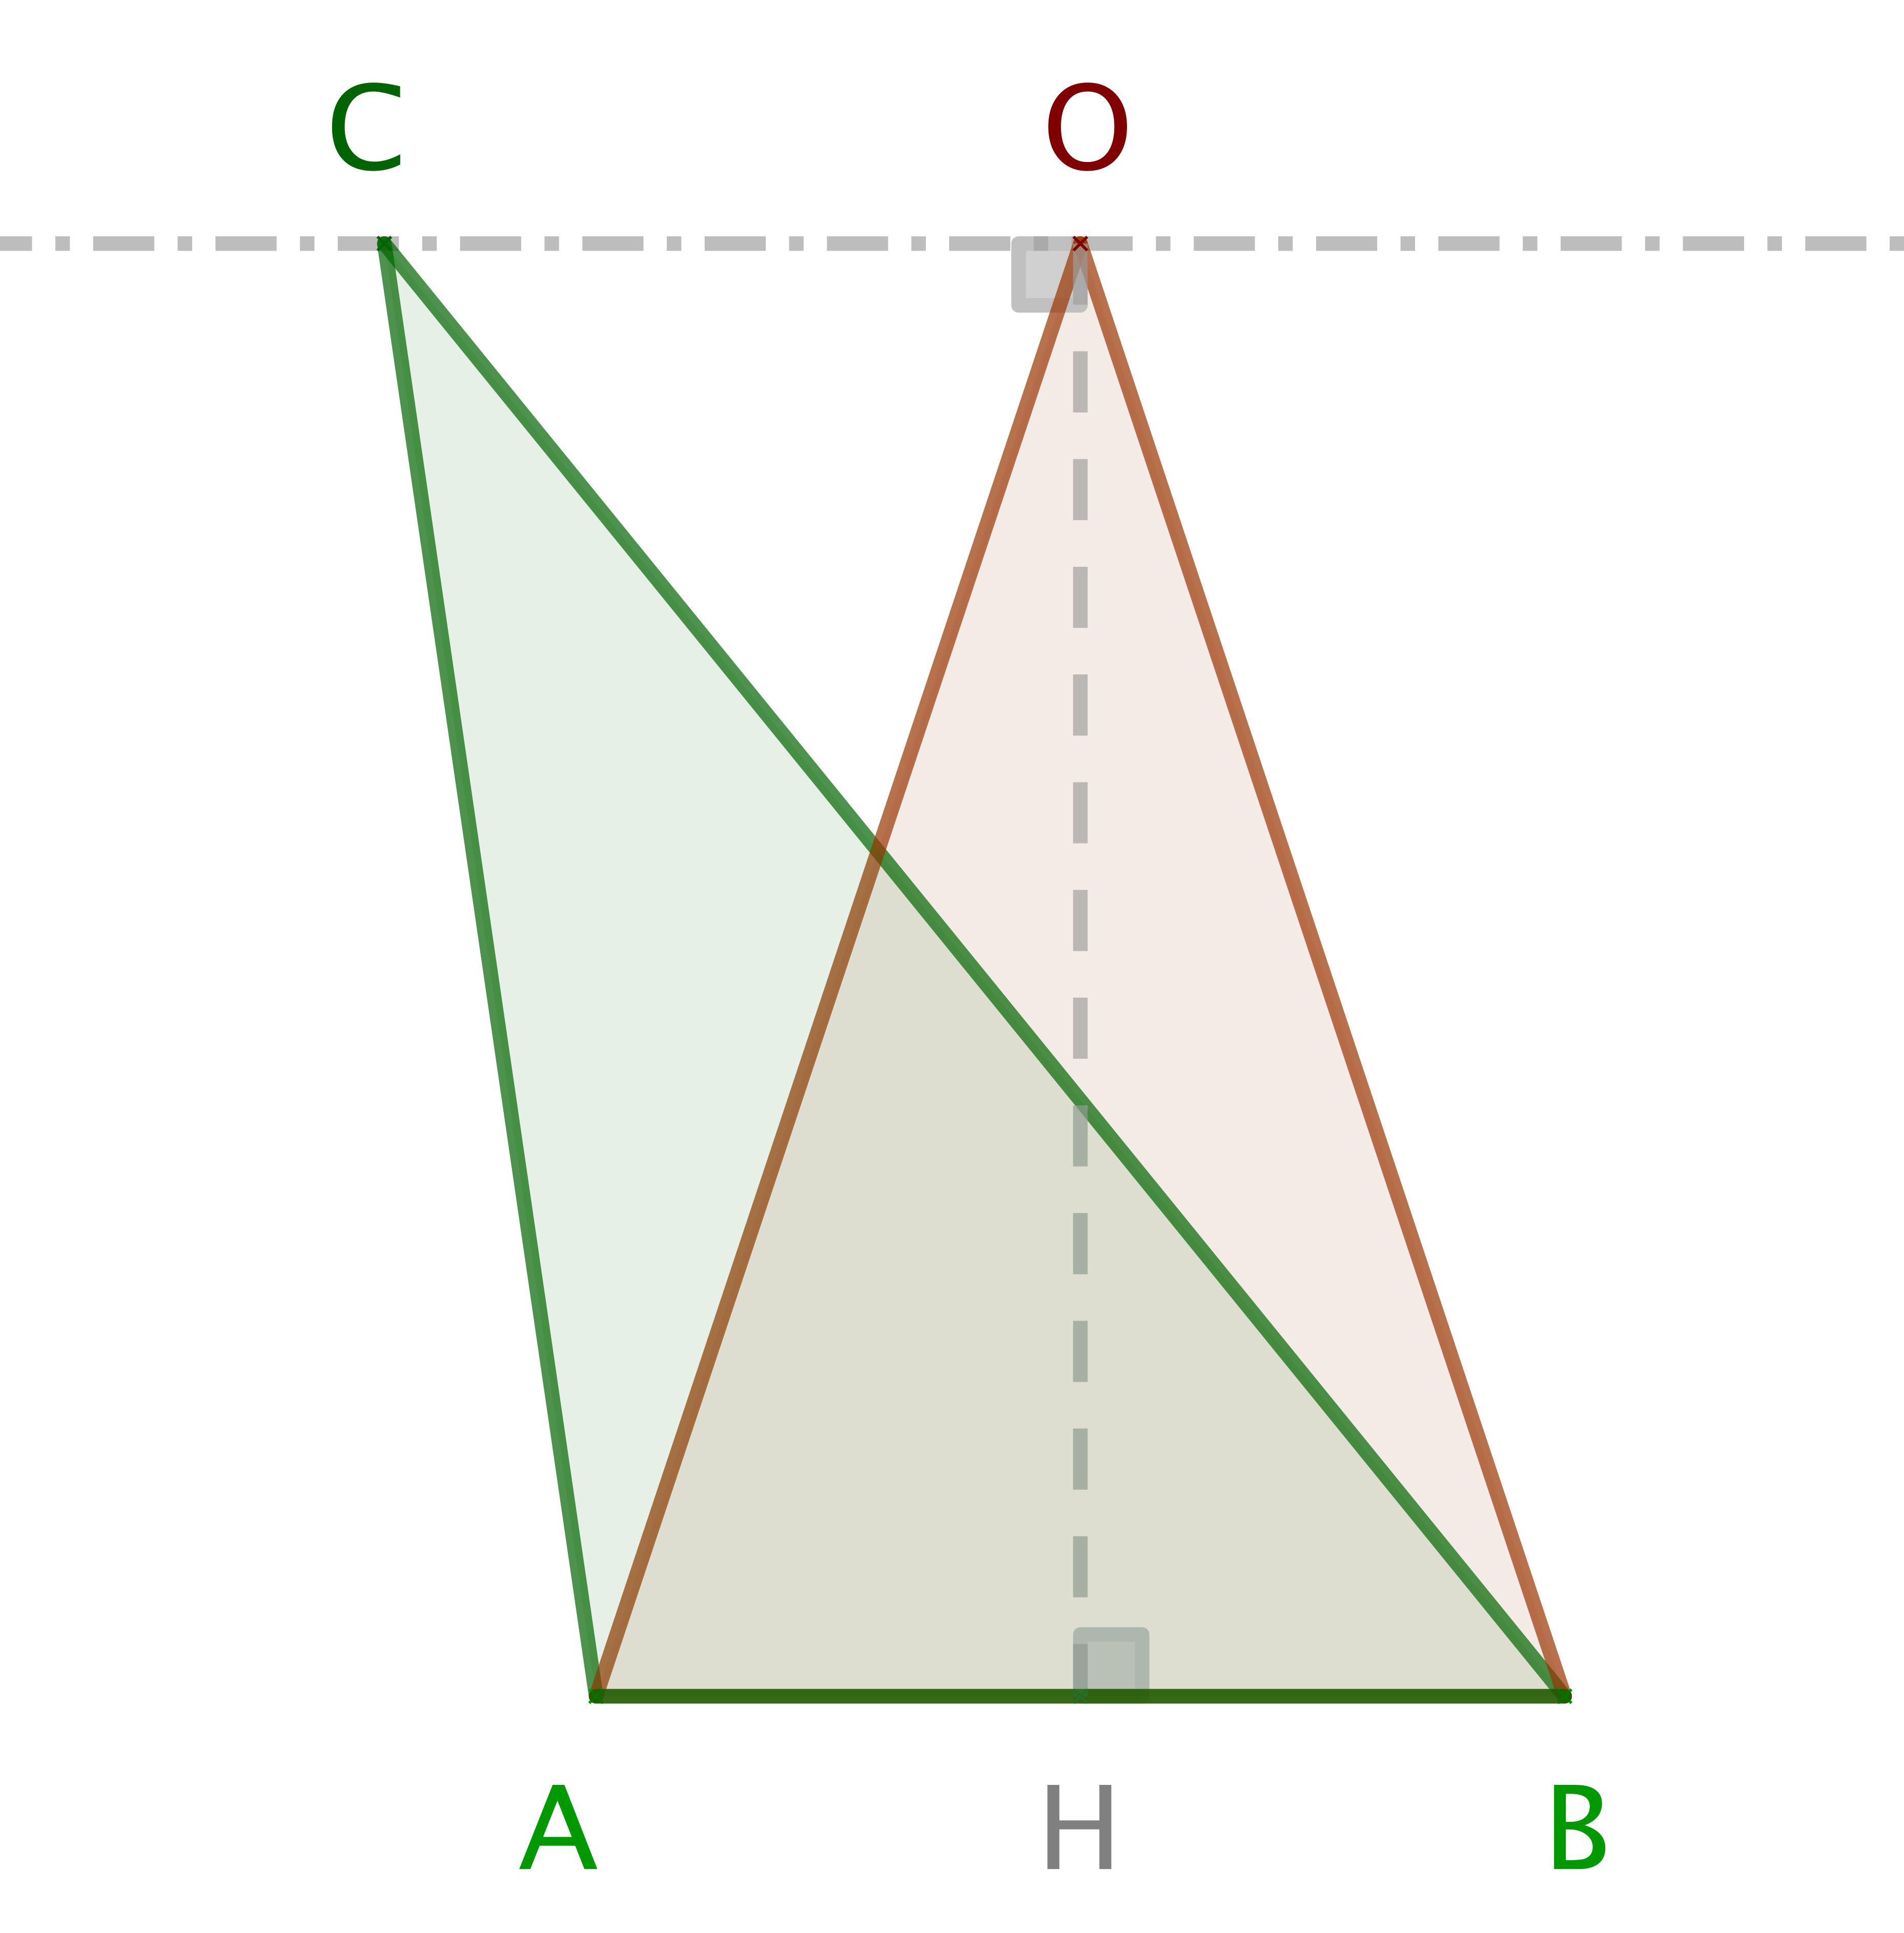
\includegraphics[scale=.4]{content/triangle/triangle.png}
	\end{center}

	Via une petite symétrie axiale, voir ci-dessous, il est aisé de noter que $\perim{ABC} \geq \perim{ABO}$.
	
	
	\begin{center}
		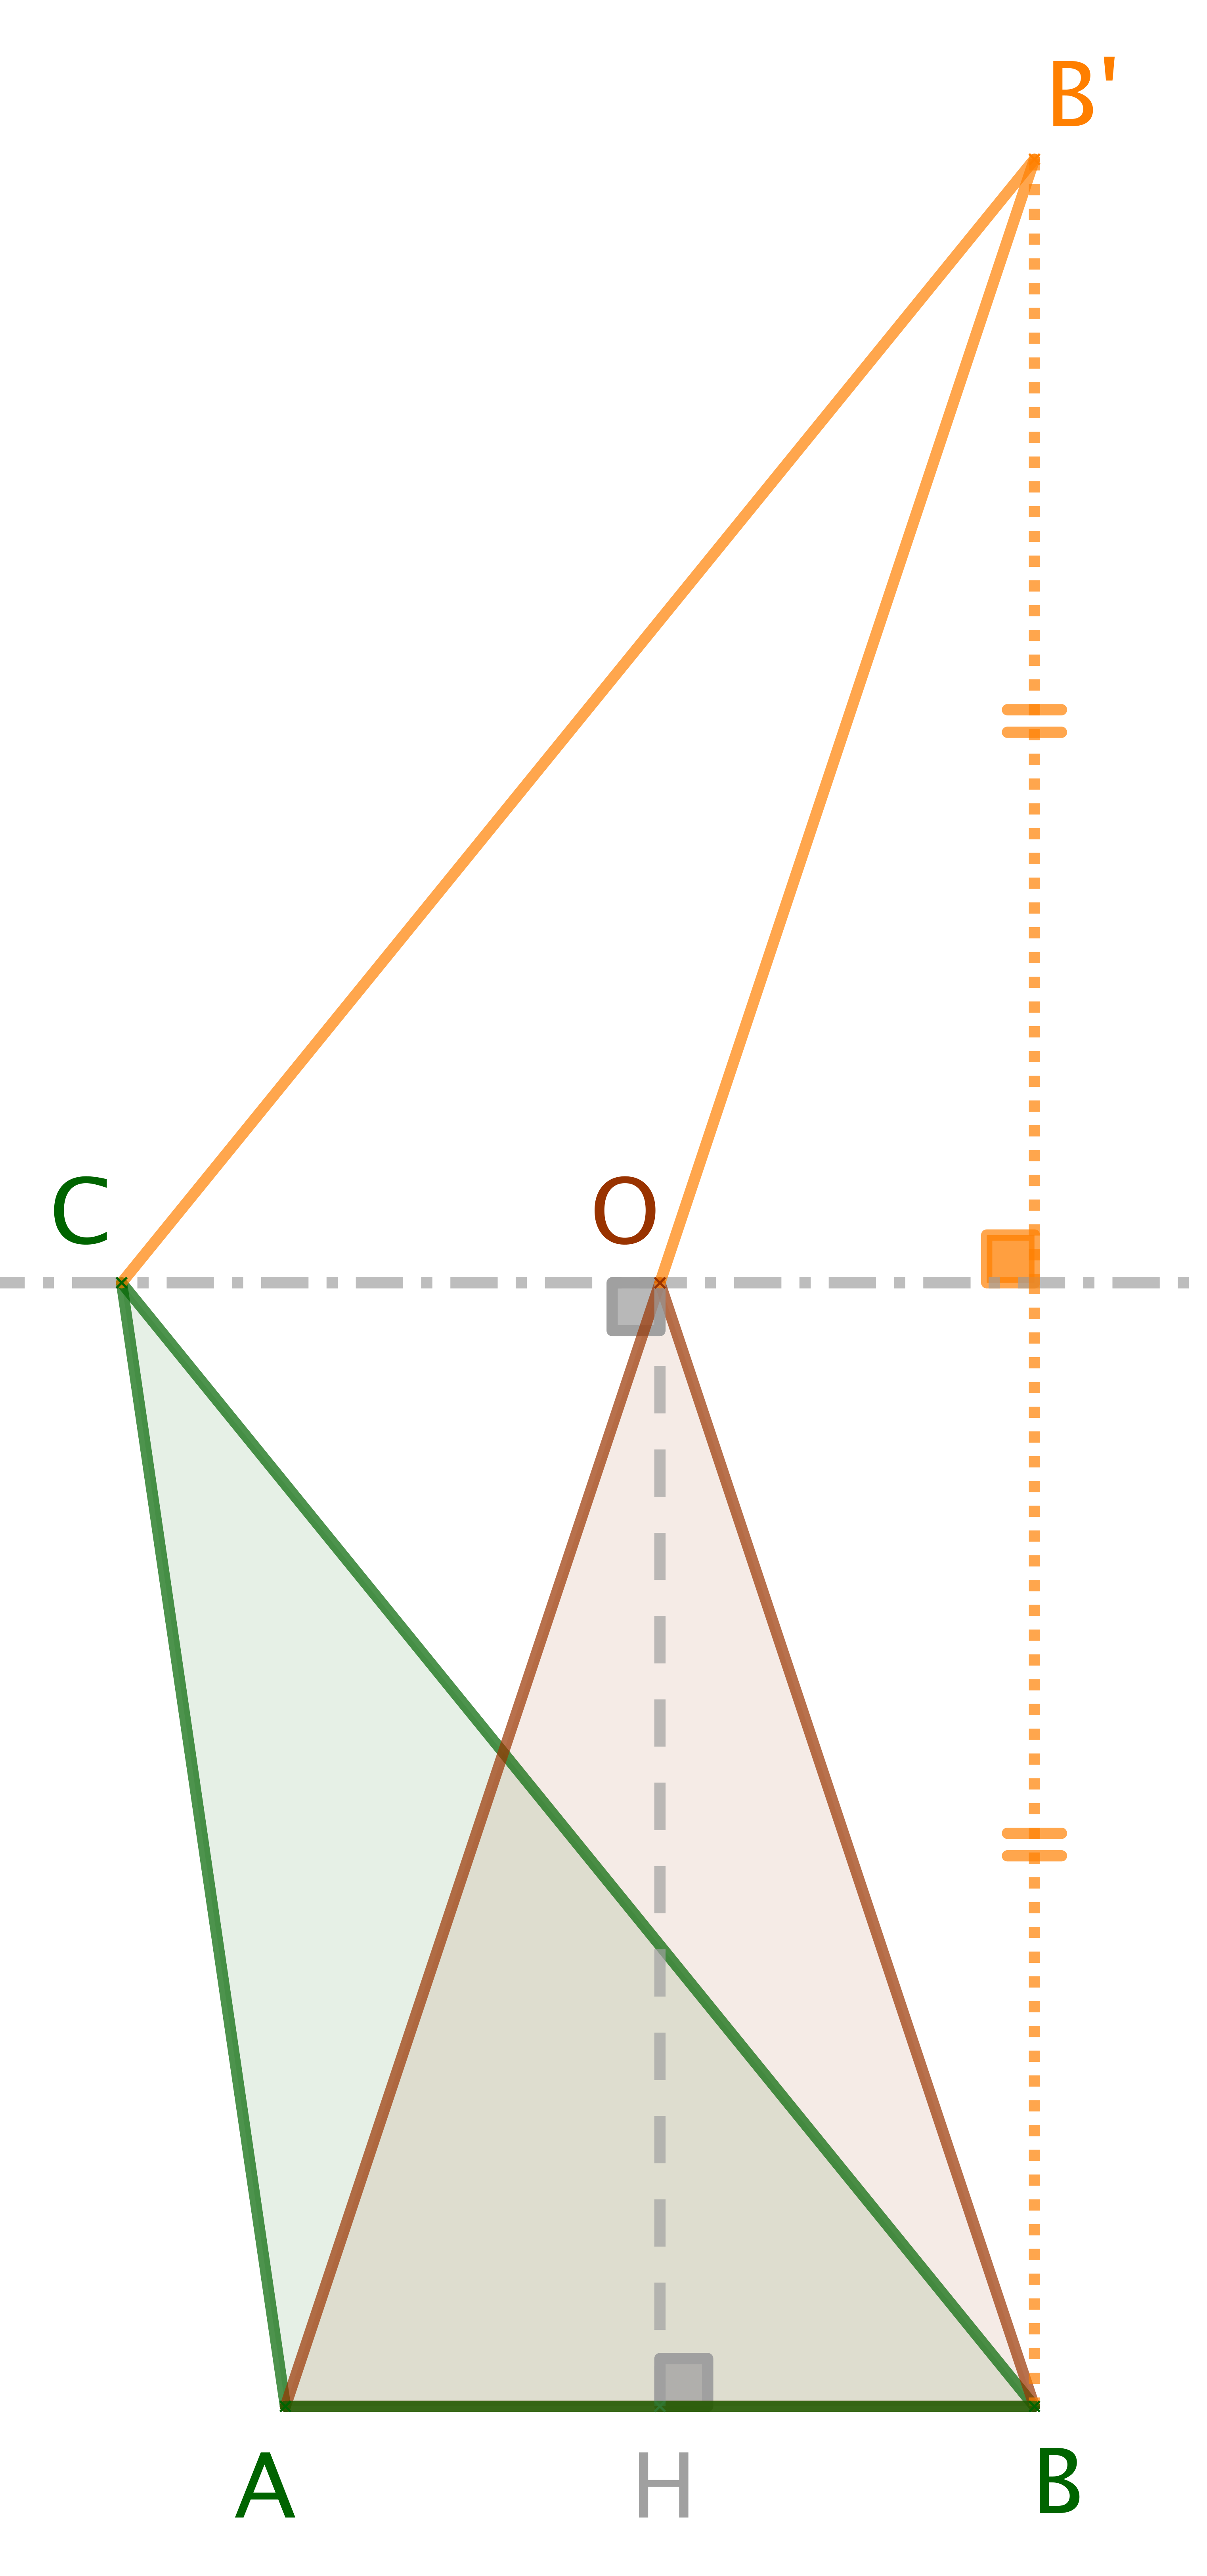
\includegraphics[scale=.4]{content/triangle/triangle-proof.png}
	\end{center}
	
	Via une dilatation verticale de rapport $r \geq 1$, on obtient finalement un triangle isocèle $ABO^{\,\prime}$ de périmètre $p$ tel que $\area{ABO^{\,\prime}} \geq \area{ABC}$.
	\footnote{
		Il est immédiat d'adapter les arguments de la méthode des extrema liés pour le triangle général au cas qui nous a occupé dans cette preuve.
	}
	Contrat rempli!
\end{proof}